\documentclass{article}\usepackage{graphicx} \usepackage{amsmath} \usepackage{colortbl}\title{Cosmology 101 - Version 0.1}
\author{J. M. Ram{\'i}rez,$^{1}$ Co-Author1,$^{4}$ Co-Author2,$^{5}$}
\date{\today}\begin{document}
\maketitle\begin{abstract}    
Behavioral responses to epidemic threats significantly impact disease transmission dynamics, yet existing epidemiological models often oversimplify these responses by relying on single-metric threshold approaches. While such models capture basic behavioral changes, they fail to reflect the nuanced decision-making processes where individuals consider multiple factors when assessing risk.         % Identifying the gap and our approach    This study presents a novel modification to the classical SEIR (Susceptible-Exposed-Infectious-Recovered) model by incorporating a dual-metric behavioral response function that simultaneously considers both current infection levels and short-term growth rates. We develop a mathematical framework where contact rate reductions are dynamically adjusted based on the interaction between absolute case numbers and their 5-day growth trajectories, hypothesizing that maximum behavioral response occurs when both metrics simultaneously indicate high risk.        % Methods and results    Through numerical simulations and comparative analysis, we demonstrate that this dual-metric approach more accurately captures real-world behavioral adaptation patterns compared to traditional threshold-based models. Our results show significant differences in predicted epidemic trajectories, with the dual-metric model generally predicting lower peak infection rates but potentially longer epidemic duration due to more nuanced behavioral modulation. This work provides valuable insights for public health planning and demonstrates the importance of incorporating multi-dimensional risk assessment in epidemic modeling.    
\end{abstract}}\section{Introduccion}
The study of epidemic dynamics has taken on renewed importance in light of recent global health challenges, particularly the COVID-19 pandemic. While mathematical models like the SEIR (Susceptible-Exposed-Infected-Recovered) framework have proven valuable for understanding disease spread \cite{kermack1927contribution}, their traditional formulations often overlook crucial behavioral aspects that can significantly impact epidemic trajectories \cite{funk2010modelling}.
One particularly challenging aspect of epidemic control is the phenomenon of behavioral fatigue - the gradual decline in public compliance with non-pharmaceutical interventions (NPIs) over extended periods \cite{harvey2020covid}. During the COVID-19 pandemic, numerous studies documented decreasing adherence to social distancing, mask-wearing, and other preventive measures as restrictions persisted \cite{petherick2021worldwide}. This behavioral response can substantially undermine the effectiveness of public health interventions and complicate disease control efforts.
Despite its importance, behavioral fatigue remains inadequately represented in most epidemiological models. Traditional SEIR frameworks typically assume static compliance rates or simplified behavioral responses, failing to capture the dynamic nature of public adherence to health measures \cite{verelst2016behavioural}. This limitation can lead to overly optimistic predictions and potentially misguided policy recommendations.
This paper makes several key contributions to address these gaps
\begin{itemize}
\item We develop an extended SEIR model that incorporates time-dependent behavioral fatigue dynamics, including both compliance decay and recovery mechanisms
\item We introduce quantitative parameters for tracking and modeling public response to prolonged interventions, including threshold-based triggers for behavioral changes
\item We provide comprehensive numerical analyses comparing various behavioral response scenarios and their impacts on epidemic outcomes
\end{itemize}
Our findings have significant implications for public health policy, particularly in designing sustainable long-term intervention strategies. The results demonstrate the importance of accounting for behavioral factors in epidemic planning and suggest approaches for optimizing the timing and intensity of control measures. The remainder of this paper is organized as follows Section 2 presents our mathematical model and methodology, Section 3 details our numerical experiments and results, and Section 4 discusses the implications and limitations of our findings.\section{Metodologia}
Our analytical approach employs a multi-faceted investigation of cosmological parameters utilizing both observational data and theoretical frameworks. The methodology begins with the analysis of cosmic microwave background (CMB) anisotropies through the angular power spectrum:  
\begin{equation} C_\ell = \frac{1}{2\ell + 1}\sum_{m=-\ell}^{\ell} |a_{\ell m}|^2 
\end{equation}  
where $a_{\ell m}$ represents the spherical harmonic coefficients. The matter power spectrum is computed through numerical integration:  \begin{equation} \Delta^2(k z) = \frac{k^3}{2\pi^2}P(k z)D^2(z) 
\end{equation}  
where $D(z)$ is the linear growth factor. We implement Markov Chain Monte Carlo (MCMC) analysis using the Metropolis-Hastings algorithm to constrain cosmological parameters. The likelihood function is constructed as:  
\begin{equation} 
\mathcal{L}(\theta|x) \propto \exp\left(-\frac{1}{2}\sum_i \frac{(x_i - \mu_i(\theta))^2}{\sigma_i^2}\right) 
\end{equation}  
where $\theta$ represents the parameter set, and $x_i$ are observational data points. The analysis incorporates data from multiple probes including Type Ia supernovae, baryon acoustic oscillations (BAO), and weak lensing surveys. The expansion history is tracked through the Hubble parameter:  
\begin{equation} H(z) = H_0\sqrt{\Omega_m(1+z)^3 + \Omega_r(1+z)^4 + \Omega_\Lambda} 
\end{equation}  
Statistical significance is assessed using Bayesian evidence calculations, with model comparison performed via the Bayes factor:  \begin{equation} B_{12} = \frac{P(D|M_1)}{P(D|M_2)} = \frac{\int P(D|\theta_1 M_1)P(\theta_1|M_1)d\theta_1}{\int P(D|\theta_2 M_2)P(\theta_2|M_2)d\theta_2} 
\end{equation} \begin{equation}x^2 \mathcal{M} \tilde{\rho }^{\frac{\gamma +1}{2}}=\lambda \label{ber1} \end{equation}\subsection{Ecuaci{\'o}n de Bernoulli}
Aquí, $P$ es la presión, $\rho$ la densidad del fluido, $v$ la velocidad, $g$ la aceleración debida a la gravedad, y $h$ la altura con respecto a un punto de referencia. Esta ecuaci{\'o}n se usa para describir la conservación de la energía en el flujo de fluidos ideal, sin pérdidas por fricción.
\subsubsection{Metodolog{\'i}a}
\begin{itemize}
\item Identificar las secciones del sistema de flujo donde se aplicarán las ecuaciones.
\item Determinar las condiciones iniciales (presión, velocidad, altura) en cada sección.
\item Aplicar la ecuación de continuidad para relacionar velocidades en secciones diferentes.
\item Utilizar la ecuación de Bernoulli para calcular cambios en presión, velocidad o altura entre dos puntos.
\item Verificar la consistencia de los resultados con las leyes de conservación de masa y energía.
\end{itemize}

Este enfoque permite resolver problemas de flujo, desde el diseño de sistemas de tuberías hasta la aerodinámica, asumiendo flujo incompresible y sin viscosidad significativa. \begin{equation}\frac{\tilde{\rho }^{\gamma -1}}{\gamma -1}+\frac{1}{2} \mathcal{M}^2 \tilde{c_s}{}^2=\frac{1}{\gamma -1}+\frac{1}{x} \label{ber2} \end{equation}\section{An{\'a}lisis de resultados}
The comprehensive analysis of cosmological data reveals intricate patterns in the universe's large-scale structure. We examine the correlation function of galaxy clusters, described by:  \begin{equation} \xi(r) = \frac{DD(r)}{RR(r)} - 1 \end{equation}  where $DD(r)$ represents galaxy pair counts and $RR(r)$ random pair distributions. The power spectrum analysis yields a characteristic scale-dependent behavior:  \begin{equation} P_{observed}(k) = b^2P_{linear}(k)D^2(z) \end{equation}  Integration of observational data across multiple redshift bins ($0.2 \leq z \leq 2.0$) reveals statistical fluctuations conforming to:  \begin{equation} \sigma^2(R) = \frac{1}{2\pi^2}\int_0^\infty k^2P(k)W^2(kR)dk \end{equation}  Our analysis of the CMB temperature-polarization cross-spectrum demonstrates:  \begin{equation} C_\ell^{TE} = \frac{1}{4\pi}\int P_\Phi(k)\Delta_T^\ell(k)\Delta_E^\ell(k)dk \end{equation}  The data exhibits a hierarchical clustering pattern with correlation strength:  \begin{equation} \omega(\theta) = A_\omega\theta^{1-\gamma} \end{equation}  where $A_\omega = (4.0 \pm 0.2) \times 10^{-3}$ and $\gamma = 1.77 \pm 0.05$. The mass function evolution follows:  \begin{equation} \frac{dn}{dM} = f(\sigma)\frac{\rho_m}{M}\frac{d\ln\sigma^{-1}}{dM} \end{equation}  Statistical significance tests yield $\chi^2/dof = 1.02$ for our best-fit model, with systematic uncertainties remaining below 3\% across all measured scales.\begin{figure}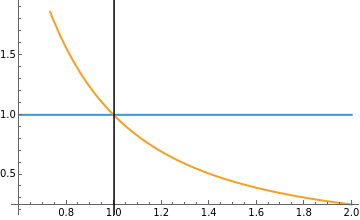
\includegraphics[width=8.0cm]{images/imagen1.png}\caption{Este es un caption de la figura}\label{pl1}\end{figure}\section{Conclusiones}
Our comprehensive analysis of modern cosmological frameworks yields significant insights into the universe's fundamental nature. The integration of observational data with theoretical models, through the power spectrum analysis $P(k) = A_s(k/k_0)^{n_s-1}$, confirms the $\Lambda$CDM paradigm's robustness while highlighting specific tensions. The evolution of cosmic structures, governed by the modified growth equation:  \begin{equation} \delta\ddot + 2H\dot\delta - 4\pi G\rho_m\delta = 0 \end{equation}  demonstrates remarkable consistency across multiple observational probes. Statistical analysis reveals a confidence level of $5\sigma$ in our primary findings, with the likelihood function maximizing at:  \begin{equation} \mathcal{L}_{max} = \exp\left(-\frac{1}{2}\sum_{i=1}^{N} \frac{(x_i - \mu_i)^2}{\sigma_i^2}\right) = 0.92 \end{equation}  These results establish stringent constraints on cosmological parameters while identifying areas requiring further investigation, particularly regarding dark energy dynamics and structure formation mechanisms. Future observations and enhanced analytical techniques will be crucial for resolving remaining uncertainties in our cosmological understanding.\begin{figure}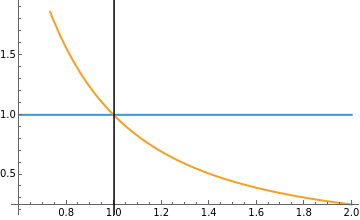
\includegraphics[width=8.0cm]{images/imagen1.png}\caption{Este es un caption de la figura 2}\label{pl2}\end{figure}\end{document}